\label{unary}

%описание оператора и принципа
В силу того, что унарный несмещенный оператор может изменять только один случайный бит в векторе, в модели генетических алгоритмов он представляет собой оператор мутации. 

\begin{figure}[H]
 }\label{fig2}
    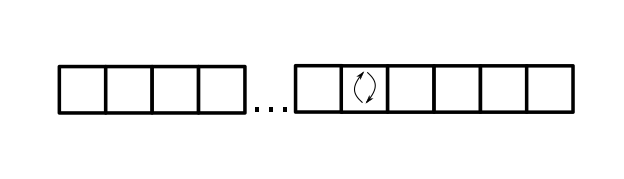
\includegraphics[height=4cm]{ITMO/pic/un.png}
\end{figure}

Разобъем все пространство поиска на некоторые классы векторов, где каждый шаг - это расстояние между первоначальным вектором и векторами этого множетсва, то есть, количество отличающихся бит. Классы будут генерироваться слеующим образом: 
\begin{itemize}
   \item $q_0$ $\leftarrow$ random
   \item $D_1$ - класс решений, отличающихся от первоначальной особи на 1 бит, размер множества n
   \item $D_2$ - размер ${n}\choose{2}$
   \item $D_3$ ...
   \item ...
   \item $D_{n-1}$ - размер ${n}\choose{n - 1}$ = n
   \item $D_n$ - размер 1, \bar{q_0}
\end{itemize} 

Введем следующее: $E(d, i)$ - матожидание от числа различных запросов на расстояние d, если на этом расстоянии сделано i запросов.

\newtheorem{theorem}{Теорема}
\begin{myth}
Даны непересекающиеся множества $S_1, ... S_k$ размеров $n_1 ... n_k$.
В одном из множеств находится элемент x. Утверждается, что в этой постановке при отсутствии другой информации, оптимизационный алгоритм выглядит так: 
\begin{algorithm}[H]
\caption{Унарный алгоритм}\label{lst1}
\begin{algorithmic}
        \For{i = 0, ... , k}
	    \State Храним $t_1 ... t_k$ - сколько запросов было сделано к соответствующему множеству
	    \State На определенном шаге вычисляем $E[z_i] = (\frac{n_i - 1}{n_i})^{t_i}$
	    \State Выбираем множество i c максимальным $E[z_i]$ и делаем запрос к этому множеству.
	    \EndFor
\end{algorithmic}
\end{algorithm}
\end{myth}
\begin{proof}
    Пусть мы знаем, сколько уникальных элементов $u_1...u_k$ было запрошено из каждого множества. Известно что количество элементов будет меньше или равно числу запросов к множеству. ($u_i \leq t_i$). 
    
    Пусть x - искомый экземпляр данной задачи, находится соответственно в одном из множеств. Предположим, что элемент x раньше не возвращался из запросов (так как при возвращении искомого элемента функция бы завершилась).
    
    
    $P_i$ = [вероятность, что $x$ лежит в $i$] = $\frac{t_i - u_i}{\sum_{j}{t_j - u_j}}$ 
    
    $p_i$ = [вероятность, что на запросе к i вернут k] = $\frac{1}{n_i} \cdot P_i$ = $\frac{n_i - u_i}{\sum_{j}{t_j - u_j}}$
    
    Так как $u_i$ - величина переменная а каждом шаге, можем посчитать матожидание в таком формате: $u_i \sim E(u_i(n_i, t_i))$
    
    До запроса было x уникальных запросов, после запроса будет: $$x + \frac{n - x}{n} = 1 + x \cdot (1 - \frac{1}{n_i})$$ 
    
    Таким образом: $E[u(n_i, t_i)] = 1 + E[u_i(n_i, t_{i} - 1)] \cdot (1 - \frac{1}{n_i})$
    
    Для $ t_i = 0 \to 0 $ - база индукции.
    
    Рассмотрим переход: 
    $E[u(n_i, t_i)]$ = $\frac{{n_i}^{ti} - {(n_i - 1)}^{ti}}{{n_i}^{t_i - 1}}$  = 1 + $[ \frac{{n_i}^{ti} - {(n_i - 1)}^{t_i}}{{n_i}^{t_i}} ] \cdot (\frac{1}{n_i})$ = $ \frac{{n_i}^{ti + 1} - {(n_i - 1)}^{t_i + 1}}{{n_i}^{t_i}} $ 
    
    Таким образом мы получаем значение, равное количеству строк на следующем шагу, а значит, теорема доказана.

\end{proof}

%здесь будет вставка от Дена для увеличения объема работы. Не знаю, пригодится ли дальше это, но пока пусть будет.


Для дальнейшего использования введем дополнительнно несколько дополнительных материалов.

\textbf{Лемма}

Дана последовательность множеств неотрицательных вещественных чисел $\{a_i^j\}_{i \in X, j \in N}$.

Тогда верно, что $$\inf_{i \in X} \lim_{j \to +\infty} a_i^j \ge \lim_{j \to +\infty} \inf_{i \in X} a_i^j$$.

\textbf{Доказательство}

По определению инфимума:

$$a_i^j \ge \inf_{k \in X} a_k^j \forall i, j$$

Тогда по предельному переходу в неравенствах (если члены одной последовательности не превосходят членов другой последовательности, то и предел первой не превосходит предел второй):

$$\lim_{j \to +\infty} a_i^j \ge \lim_{j \to +\infty} \inf_{k \in X} a_k^j \forall i$$

Так как это верно для любого $i$, то неравенство остается верным, если слева взять инфимум по всем $i$:

$$\inf_{i \in X} \lim_{j \to +\infty} a_i^j \ge \lim_{j \to +\infty} \inf_{i \in X} a_i^j$$

лемма доказана

\newtheorem{theorem}{Теорема}
\begin{myth}
Пусть даны две бесконечные последовательности $\{a_i\}_{i = 0}^{+\infty}$ и $\{b_i\}_{i = 0}^{+\infty}$.

Пусть при этом первая может быть упорядочена по возрастанию (для любого элемента множество меньших элементов конечно), а вторая -- по убыванию (для любого элемента конечно множество больших элементов).

Тогда в случае сходимости ряда $\sum_{i = 0}^{+\infty} a_i b_i$ минимальное значение его суммы достигается, когда первая последовательность отсортирована по возрастанию, а вторая -- по убыванию
\end{myth}

\begin{proof}
    

Будем считать, что $\{b_i\}_{i = 0}^{+\infty}$ уже упорядочена по возрастанию (это можно сделать вследствие того, что смена порядка членов ряда с неотрицательными членами не меняет его суммы). Тогда нам требуется только найти перестановку $\{a_i\}$, минимизирующую их скалярное произведение. Далее для краткости вместо $\inf_{\textit{for all permutations of }a_i}$ будем писать просто $\inf$.

Итак, по определению ряда:

$$\inf \sum_{i = 0}^{+\infty} a_i b_i = \inf \lim_{n \to +\infty} \sum_{i = 0}^{n} a_i b_i.$$

По лемме:

$$\inf \lim_{n \to +\infty} \sum_{i = 0}^{n} a_i b_i \ge \lim_{n \to +\infty} \inf \sum_{i = 0}^{n} a_i b_i.$$

Далее нам для достижения минимума надо взять минимальные $n$ элементов из $a_i$. Как легко доказать для случая не с последовательностями, а с конечномерными векторами, для достижения инфимума отсортировать их надо по возрастанию (так как $\{b_i\}$ уже отсортированы по убыванию). Тогда если $\{c_i\}$ -- отсортированная по возрастанию последовательность $\{a_i\}$, то

$$\lim_{n \to +\infty} \inf \sum_{i = 0}^{n} a_i b_i = \lim_{n \to +\infty} \sum_{i = 0}^{n} c_i b_i.$$

А по определению суммы ряда

$$\lim_{n \to +\infty} \sum_{i = 0}^{n} c_i b_i = \sum_{i = 0}^{+\infty} c_i b_i.$$

Таким образом, мы показали, что 

$$\inf \sum_{i = 0}^{+\infty} a_i b_i \ge \sum_{i = 0}^{+\infty} c_i b_i.$$

Так как правая часть является элементом множества, по которому берется инфимум слева, то она не может быть меньше, а следовательно, обе части неравенства равны. Так как $\{c_i\}$ -- отсортированная по возрастанию $\{a_i\}$, то теорема доказана.

\end{proof}

Рассмотрим все классы пространства поиска. Заметим, что так как каждый класс содержит векторы, отличающиеся на i бит от изначальной особи, то 